\documentclass[aspectratio=169]{beamer}

\usepackage[utf8]{inputenc}
\usepackage[T1]{fontenc}
\usepackage[spanish]{babel}
\usepackage{lmodern}
\usepackage{graphicx}
\usepackage{booktabs}
\usepackage{array}
\usepackage{xcolor}
\usepackage{hyperref}
\usepackage{listings}
\usepackage{amsmath}
\newcolumntype{L}[1]{>{\raggedright\arraybackslash}p{#1}}

\usetheme{Madrid}
\setbeamertemplate{navigation symbols}{}%
\definecolor{codeblue}{RGB}{0,70,140}
\definecolor{codegray}{RGB}{245,245,245}
\hypersetup{colorlinks=true, linkcolor=codeblue, urlcolor=codeblue}

\lstset{
  basicstyle=\scriptsize\ttfamily,
  keywordstyle=\color{codeblue}\bfseries,
  commentstyle=\color{gray},
  stringstyle=\color{codeblue},
  showstringspaces=false,
  frame=single,
  breaklines=true,
  backgroundcolor=\color{codegray}
}

\title[Paralelismo en C y Python]{Paralelismo en C y Python: Rendimiento en la Era Post-Dennard}
\subtitle[Paralelismo C vs. Python]{De Pthreads y OpenMP al multiprocesamiento y Joblib}
\author[Espinoza H.; Linares R.]{\texorpdfstring{Espinoza H., Diego A. \\ Linares R., Ander R.}{Espinoza H., Diego A.; Linares R., Ander R.}}
\institute[UNMSM -- Grupo 10]{\texorpdfstring{Universidad Nacional Mayor de San Marcos \\ Grupo 10}{UNMSM -- Grupo 10}}
\date{2025}

\begin{document}

\begin{frame}
  \titlepage
\end{frame}

\begin{frame}{Agenda}
  \tableofcontents
\end{frame}

\AtBeginSection[]{
  \begin{frame}{Ruta}
    \tableofcontents[currentsection]
  \end{frame}
}

\section{Introducción}

\begin{frame}{Motivación y audiencia}
  \begin{itemize}
    \item Fin del escalado de Dennard: más núcleos en lugar de frecuencias crecientes.
    \item Curso de Redes, Arquitectura y Comunicaciones dirigido a estudiantes de la Facultad de Ciencias Matemáticas.
    \item Objetivo: mostrar patrones prácticos de paralelismo con énfasis en código real y decisiones de diseño.
  \end{itemize}
\end{frame}

\begin{frame}{Imperativo del paralelismo}
  \begin{itemize}
    \item Multinúcleo obliga a dividir trabajo en flujos simultáneos para servidores, procesamiento de paquetes y cómputo intensivo.
    \item Lenguajes presentan filosofías distintas: C ofrece control de bajo nivel; Python prioriza productividad y simplicidad.
    \item El diseño debe balancear latencia, throughput y complejidad de implementación.
  \end{itemize}
\end{frame}

\begin{frame}{Contexto visual}
  \begin{figure}
    \centering
    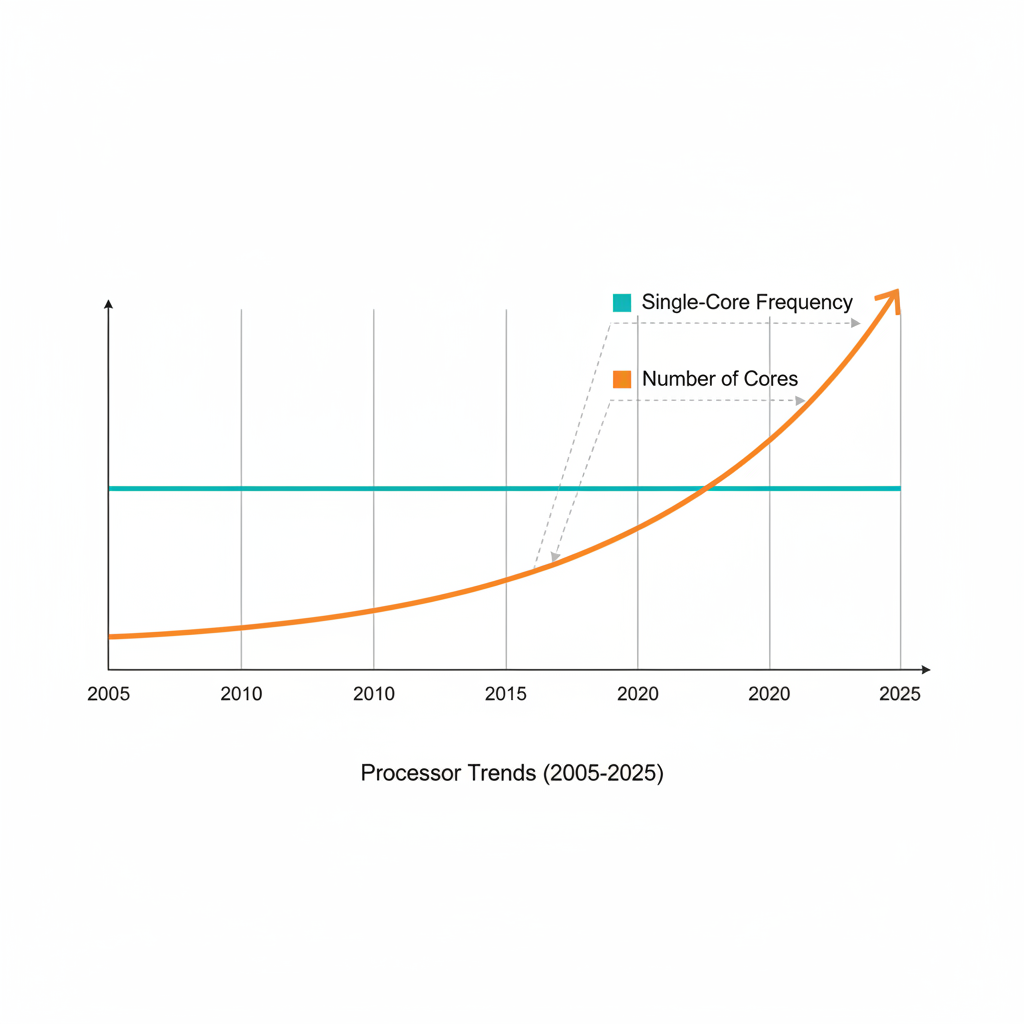
\includegraphics[height=0.6\textheight]{img/01-frecuencia-vs-nucleos.png}
    \caption{Crecimiento de la frecuencia de un solo núcleo frente al número de núcleos.}
  \end{figure}
\end{frame}

\section{Concurrencia vs. Paralelismo}

\begin{frame}{Definiciones clave}
  \begin{itemize}
    \item Concurrencia: múltiples tareas progresan de forma intercalada; ideal para E/S y ocultar latencia.
    \item Paralelismo: ejecución simultánea real en núcleos distintos; requiere hardware multiprocesador.
    \item En Python los hilos son concurrentes por el GIL; en C los hilos pueden ser concurrentes y paralelos.
  \end{itemize}
\end{frame}

\begin{frame}{Uso recomendado}
  \begin{itemize}
    \item E/S intensiva: concurrencia con hilos o async para mantener alta utilización de CPU.
    \item Carga CPU: dividir dominios de datos y mapearlos a núcleos mediante hilos nativos o procesos.
    \item Riesgos: condiciones de carrera y errores de partición (off-by-one) si no se planifica el rango de trabajo.
  \end{itemize}
\end{frame}

\begin{frame}{Ilustración conceptual}
  \begin{figure}
    \centering
    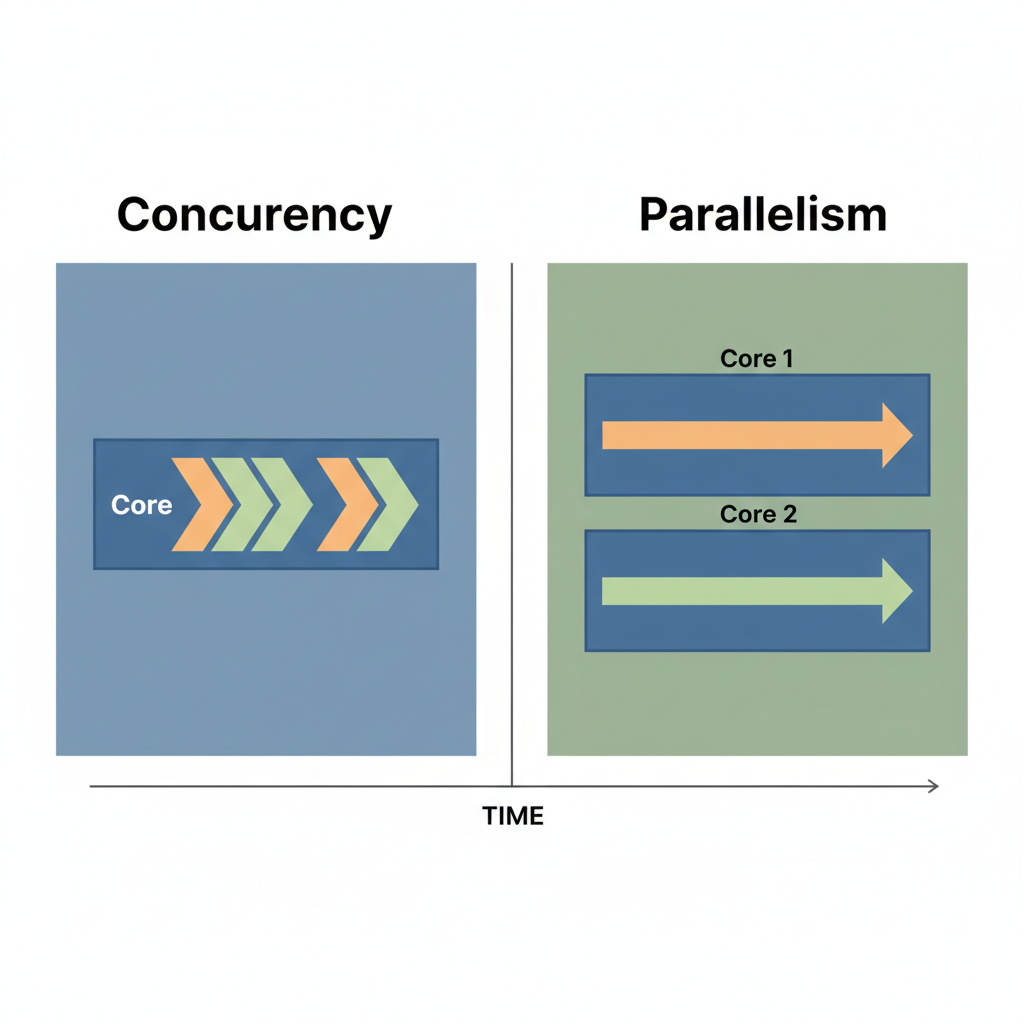
\includegraphics[height=0.6\textheight]{img/02-concurrencia-vs-paralelismo.png}
    \caption{Concurrencia vs. Paralelismo.}
  \end{figure}
\end{frame}

\section{Modelos de Memoria}

\begin{frame}{UMA vs. NUMA}
  \begin{table}
    \centering
    \begin{tabular}{@{}L{0.3\textwidth}L{0.28\textwidth}L{0.28\textwidth}@{}}
      \toprule
      & \textbf{UMA} & \textbf{NUMA} \\
      \midrule
      Memoria & Espacio compartido uniforme & Bancos locales por CPU \\
      Latencia & Constante & Depende de la distancia \\
      Escalabilidad & Limitada por bus & Alta con interconexiones rápidas \\
      C & Acceso plano; posible afinidad opcional & Requiere pinning para evitar saltos remotos \\
      Python & Copia de datos en procesos & Multiprocessing puede aislar procesos por nodo \\
      \bottomrule
    \end{tabular}
  \end{table}
\end{frame}

\begin{frame}{Implicaciones prácticas}
  \begin{itemize}
    \item Pthreads y OpenMP comparten memoria: sincronización y coherencia de caché son críticas.
    \item Multiprocessing aísla memoria y evita condiciones de carrera, pero agrega sobrecarga por serialización IPC.
    \item NumPy y BLAS liberan el GIL y usan hilos nativos, aprovechando memoria compartida de forma eficiente.
  \end{itemize}
\end{frame}

\begin{frame}{Mapa visual}
  \begin{figure}
    \centering
    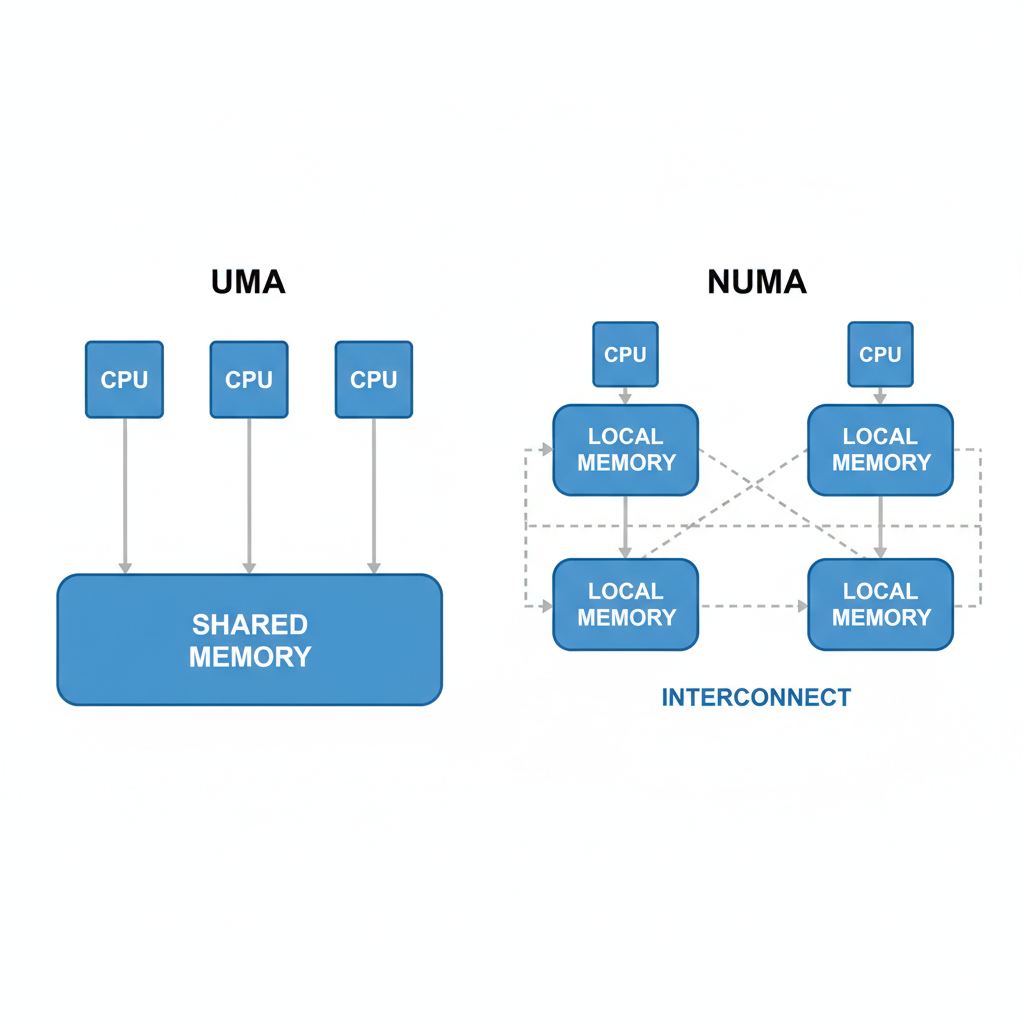
\includegraphics[height=0.6\textheight]{img/03-uma-vs-numa.png}
    \caption{Arquitecturas de memoria UMA vs. NUMA.}
  \end{figure}
\end{frame}

\section{Paralelismo en C}

\begin{frame}{Pthreads: control de bajo nivel}
  \begin{itemize}
    \item API del sistema operativo: creación, join y sincronización manual con mutexes o semáforos.
    \item Firma de hilo \texttt{void *(*start\_routine)(void *)} obliga a empaquetar argumentos y manejar castings.
    \item Partición explícita del trabajo: cálculo de \texttt{start\_row} y \texttt{end\_row} debe evitar errores off-by-one.
    \item Overhead: crear muchos hilos pequeños degrada rendimiento; conviene aproximar al número de núcleos físicos.
  \end{itemize}
\end{frame}

\begin{frame}[fragile]{Ejemplo: worker de multiplicación}
  \lstset{language=C}
  \begin{lstlisting}
typedef struct {
  int tid;
  int start_row;
  int end_row;
} thread_data_t;

void *multiply_worker(void *arg) {
  thread_data_t *data = (thread_data_t *)arg;
  for (int i = data->start_row; i < data->end_row; ++i) {
    for (int j = 0; j < N; ++j) {
      double sum = 0.0;
      for (int k = 0; k < N; ++k) {
        sum += A[i][k] * B[k][j];
      }
      C[i][j] = sum;
    }
  }
  pthread_exit(NULL);
}
  \end{lstlisting}
\end{frame}

\begin{frame}{OpenMP: directivas declarativas}
  \begin{itemize}
    \item Modelo fork-join implícito: el compilador genera hilos y sincronizaciones.
    \item Directivas como \texttt{\#pragma omp parallel for schedule(static)} distribuyen bucles sin código auxiliar.
    \item Cláusulas \texttt{private} y \texttt{shared} controlan el alcance de variables temporales y globales.
    \item \texttt{schedule(dynamic)} balancea carga irregular sin implementar colas manuales.
  \end{itemize}
\end{frame}

\begin{frame}[fragile]{Snippet OpenMP en C}
  \lstset{language=C}
  \begin{lstlisting}
#pragma omp parallel for schedule(static)
for (int i = 0; i < rows; ++i) {
  for (int j = 0; j < cols; ++j) {
    double sum = 0.0;
    for (int k = 0; k < inner; ++k) {
      sum += A[i][k] * B[k][j];
    }
    C[i][j] = sum;
  }
}
  \end{lstlisting}
\end{frame}

\section{Paralelismo en Python}

\begin{frame}{El GIL y sus efectos}
  \begin{itemize}
    \item El Global Interpreter Lock protege el conteo de referencias, permitiendo un único hilo de bytecode a la vez.
    \item En tareas CPU los hilos compiten por el GIL y pueden ser más lentos que la versión secuencial.
    \item El intérprete libera el GIL durante E/S bloqueante, por lo que el modelo sigue siendo útil para cargas I/O-bound.
  \end{itemize}
\end{frame}

\begin{frame}{Threading para E/S}
  \begin{itemize}
    \item Ideal para servidores que esperan red o disco; la latencia se oculta mientras otros hilos avanzan.
    \item Sin paralelismo real en CPU intensivo; evite usarlo para cómputo pesado.
    \item Coordine con colas o semáforos de la librería estándar para evitar condiciones de carrera en datos compartidos.
  \end{itemize}
\end{frame}

\begin{frame}[fragile]{Multiprocessing: evasión del GIL}
  \lstset{language=Python}
  \begin{lstlisting}
from multiprocessing import Pool, cpu_count

def cpu_intensive_task(n):
    return n * n

if __name__ == '__main__':
    with Pool(processes=cpu_count()) as pool:
        results = pool.map(cpu_intensive_task, range(8))
  \end{lstlisting}
  \begin{itemize}
    \item Cada proceso tiene su propio intérprete y GIL; se paga serialización de datos (pickle) e IPC.
    \item Usar bloques \texttt{if \_\_name\_\_ == '\_\_main\_\_'} evita creación recursiva de procesos en Windows.
  \end{itemize}
\end{frame}

\begin{frame}[fragile]{Joblib para ciencia de datos}
  \lstset{language=Python}
  \begin{lstlisting}
from joblib import Parallel, delayed

def process_image_stub(image_id):
    return f'Img {image_id} done'

results = Parallel(
    n_jobs=-1, prefer='processes', verbose=5
)(delayed(process_image_stub)(i) for i in range(20))
  \end{lstlisting}
  \begin{itemize}
    \item Sintaxis declarativa para pipelines intensivos en CPU; \texttt{n\_jobs=-1} usa todos los núcleos.
    \item Puede usar \texttt{memmap} para compartir arrays grandes sin copias, reduciendo la sobrecarga de pickle.
  \end{itemize}
\end{frame}

\begin{frame}{Visual del GIL}
  \begin{figure}
    \centering
    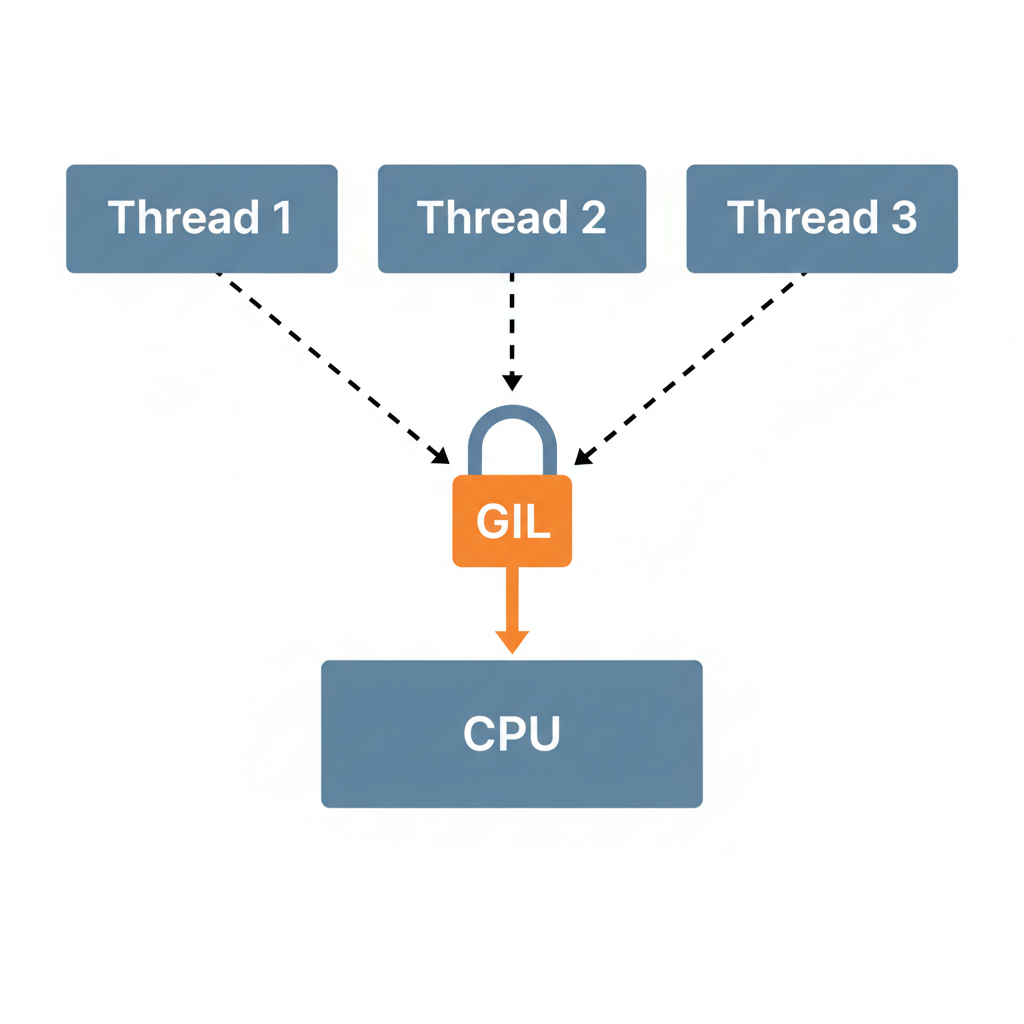
\includegraphics[height=0.6\textheight]{img/05-gil.png}
    \caption{Visualización del Global Interpreter Lock (GIL) de Python.}
  \end{figure}
\end{frame}

\section{Comparativa y Benchmarks}

\begin{frame}{Rendimiento y sobrecarga}
  \small
  \begin{tabular}{@{}L{0.35\textwidth}L{0.28\textwidth}L{0.28\textwidth}@{}}
    \toprule
    & \textbf{C/OpenMP} & \textbf{Python (multiprocessing)} \\
    \midrule
    Rendimiento CPU & Base 1.0x; acceso directo a registros & 0.1x--0.5x limitado por pickle e IPC \\
    Threading CPU & Paralelo real & Serializado por GIL \\
    Tiempo de inicio & Microsegundos (hilos ligeros) & Milisegundos (procesos) \\
    Memoria & Compartida, requiere sincronización & Copia de heap; memoria aislada \\
    Comunicación & Punteros, cero copia & Pickle por tuberías o sockets \\
    \bottomrule
  \end{tabular}
\end{frame}

\begin{frame}{Costo de desarrollo vs. ejecución}
  \begin{itemize}
    \item C/OpenMP: mayor esfuerzo de depuración y manejo de memoria; ideal para rutas críticas que se ejecutan millones de veces.
    \item Python/Joblib: itera rápido y simplifica pipelines; aceptable cuando el tiempo de pared no es crítico.
    \item Estrategia híbrida: usar Python como orquestador y bajar a extensiones en C o Numba cuando el perfil marque cuellos de botella.
  \end{itemize}
\end{frame}

\begin{frame}{Arquitectura híbrida recomendada}
  \begin{itemize}
    \item Núcleo de cómputo intensivo en C/C++ u OpenMP, liberando el GIL y aprovechando NUMA.
    \item Capa de orquestación y análisis en Python con Joblib, NumPy o Numba.
    \item Integración por FFI, extensiones o bindings para mantener un solo pipeline de entrega.
  \end{itemize}
  \begin{figure}
    \centering
    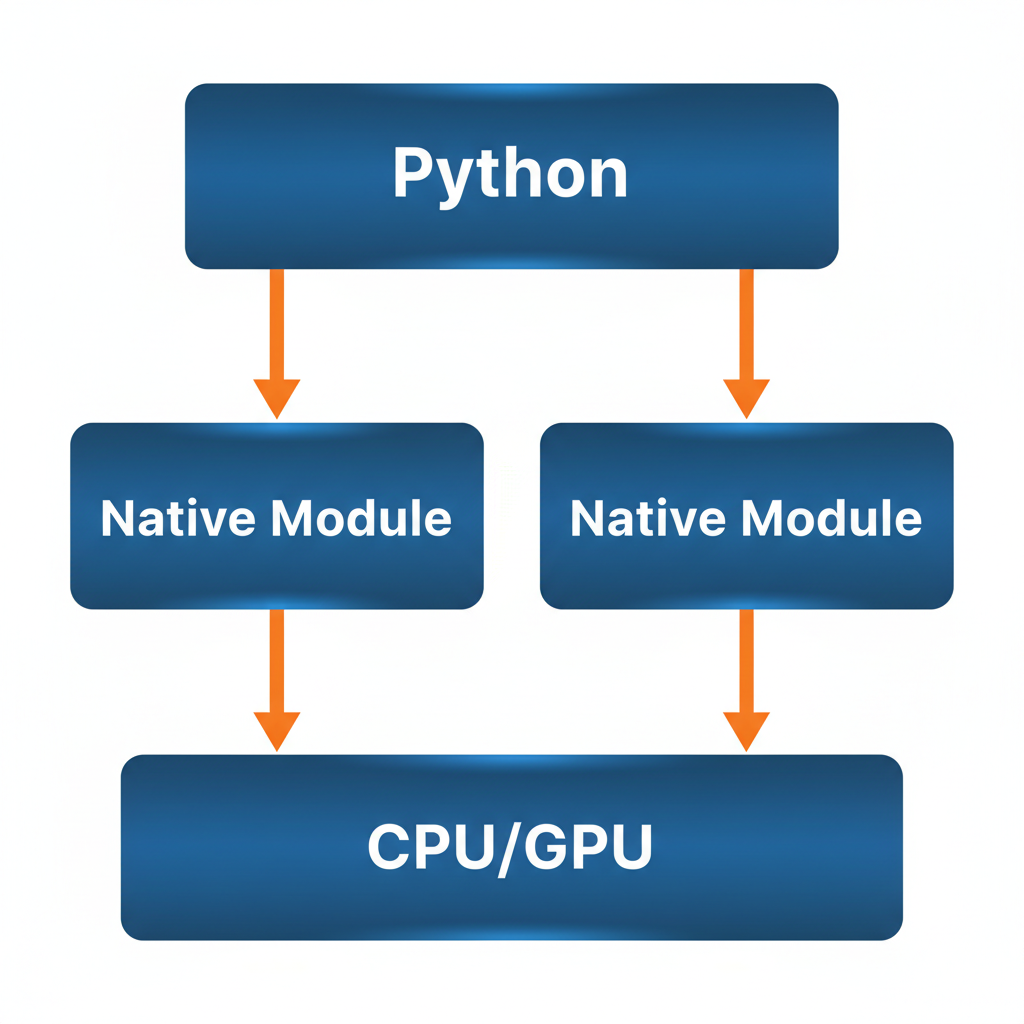
\includegraphics[height=0.45\textheight]{img/06-arquitectura-hibrida.png}
    \caption{Arquitectura híbrida con Python como orquestador.}
  \end{figure}
\end{frame}

\section{Conclusiones}

\begin{frame}{Hallazgos clave}
  \begin{itemize}
    \item El paralelismo dejó de ser opcional: la era multinúcleo obliga a dividir el trabajo en hilos o procesos.
    \item C con Pthreads u OpenMP ofrece control fino y el mayor rendimiento, pero exige disciplina en partición y sincronización.
    \item Python brilla en productividad; logra paralelismo real con procesos o delegando a librerías nativas que liberan el GIL.
    \item Elegir la herramienta depende del balance entre latencia objetivo, complejidad aceptable y ritmo de iteración de la solución.
  \end{itemize}
\end{frame}

\begin{frame}{Siguientes pasos sugeridos}
  \begin{itemize}
    \item Identificar rutas críticas en proyectos de la Facultad y perfilar su sensibilidad a la latencia.
    \item Probar versiones híbridas: prototipo en Python, optimizar kernels con OpenMP o Numba.
    \item Medir impacto de afinidad de hilos en NUMA y ajustar configuraciones de compilador o planificador.
  \end{itemize}
\end{frame}

\section{Bibliografía}

\begin{frame}[allowframebreaks]{Referencias principales}
  \begin{thebibliography}{9}
    \bibitem{pyomp}
    OpenMP. PyOMP: Parallel Multithreading that is fast and Pythonic. Disponible en \url{https://www.openmp.org/wp-content/uploads/OpenMPBoothTalk-PyOMP.pdf} (consulta: nov. 2025).

    \bibitem{cuda-numba}
    IEEE. Lessons learned from comparing C-CUDA and Python-Numba for GPU-Computing. \url{https://ieeexplore.ieee.org/document/9092407} (consulta: nov. 2025).

    \bibitem{pthreads-openmp}
    Stack Overflow. Pthreads vs. OpenMP. \url{https://stackoverflow.com/questions/3949901/pthreads-vs-openmp} (consulta: nov. 2025).

    \bibitem{iaeng}
    IAENG. Performance of Parallelism in Python and C++. \url{https://www.iaeng.org/IJCS/issues_v50/issue_2/IJCS_50_2_27.pdf} (consulta: nov. 2025).

    \bibitem{omp4py}
    arXiv. OMP4Py: a pure Python implementation of OpenMP. \url{https://arxiv.org/html/2411.14887v1} (consulta: nov. 2025).

    \bibitem{particles}
    ResearchGate. Performance Analysis of C and Python Parallel Implementations on a Multicore System Using Particle Simulation. \url{https://www.researchgate.net/publication/379138015_Performance_Analysis_of_C_and_Python_Parallel_Implementations_on_a_Multicore_System_Using_Particle_Simulation} (consulta: nov. 2025).
  \end{thebibliography}
\end{frame}

\section*{Cierre}

\begin{frame}{Gracias}
  \centering
  \vfill
  \textbf{Gracias por su atención}\\[0.5cm]
  Preguntas y comentarios son bienvenidos.
  \vfill
\end{frame}


\end{document}
